\chapter{実験2}

    \section{目的}

        実験2では,実験1で使用した刺激と同じ色度を持つ単色パッチを用いて明るさを定量化する.
        実験1の光沢感の色度による傾向と明るさの色度による傾向を比較することで,光沢感と刺激に対する明るさ感を明らかにする.


    \section{実験方法}
        \subsection{実験環境,被験者}

            実験2で用いた装置と参加した被験者は,いずれも実験1と同一であった.

        \subsection{実験刺激}

            \begin{figure}[h]
                \centering
                
\includegraphics[width=14.0cm]{./img/ex2_stimuli2.png}
                \caption{実験刺激の例}
                \label{ex2_stimuli}
            \end{figure}

            \begin{figure}[h]
                \centering
                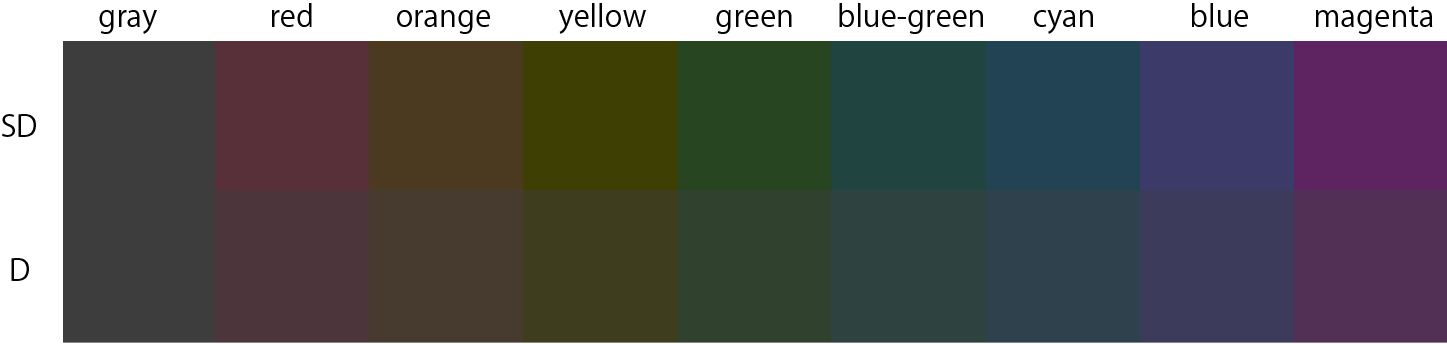
\includegraphics[width=14.0cm]{./img/ex2_stimuli_p.png}
                \caption{参照刺激として使われた色}
                \label{ex2_stimuli_set}
            \end{figure}
            \newpage

            図に実験2で使用する刺激と,参照刺激に使われた色を図\ref{ex2_stimuli}と図\ref{ex2_stimuli_set}に示す.
            参照刺激として使われた18種類の色度は,実験1で用いたDragon形状におけるSD条件,D条件のそれぞれの刺激の平均色である.

        \subsection{実験手続き}

            \begin{figure}[h]
                \centering
                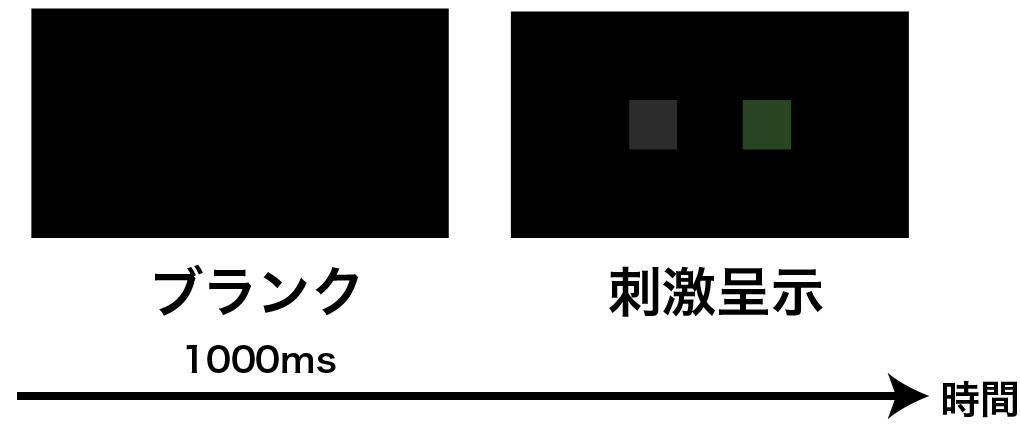
\includegraphics[width=10.0cm]{./img/ex2_procedure.png}
                \caption{1試行の流れ}
                \label{ex2_procedure}
            \end{figure}

            実験2では調整法によりカラーパッチの知覚的な明るさを計測する.
            実験2の1試行の流れを図\ref{ex2_procedure}に示す.
            各試行では,はじめに黒背景のみからなるブランク画面が 1000 ms の間呈示された.
            次に参照刺激であるカラーパッチとテスト刺激である無彩色パッチからなる刺激対が呈示された.
            被験者はトラックボールを左右に回すことにより,無彩色パッチの輝度を調節し, カラーパッチと同じ明るさに知覚されるようになるまで操作した.
            同じ明るさと判断した場合はトラックボールマウスの右クリックを押すことで次の試行のブランク画面へ移行した.
            この時,テスト刺激の輝度が記録された.
            カラーパッチと無彩色パッチの左右位置は試行ごとにランダムに決定された.

            各セッションは 2 着色条件 ✕ 色度 9 通り = 18 試行からなり,各被験者は全体で5セッションの実験を行った.
            各セッションの 18 試行で使われる参照刺激は全てランダムな順序で選ばれた.

    \section{実験結果}

        \subsection{H-K効果の大きさ}

            \begin{figure}[h]
                \centering
                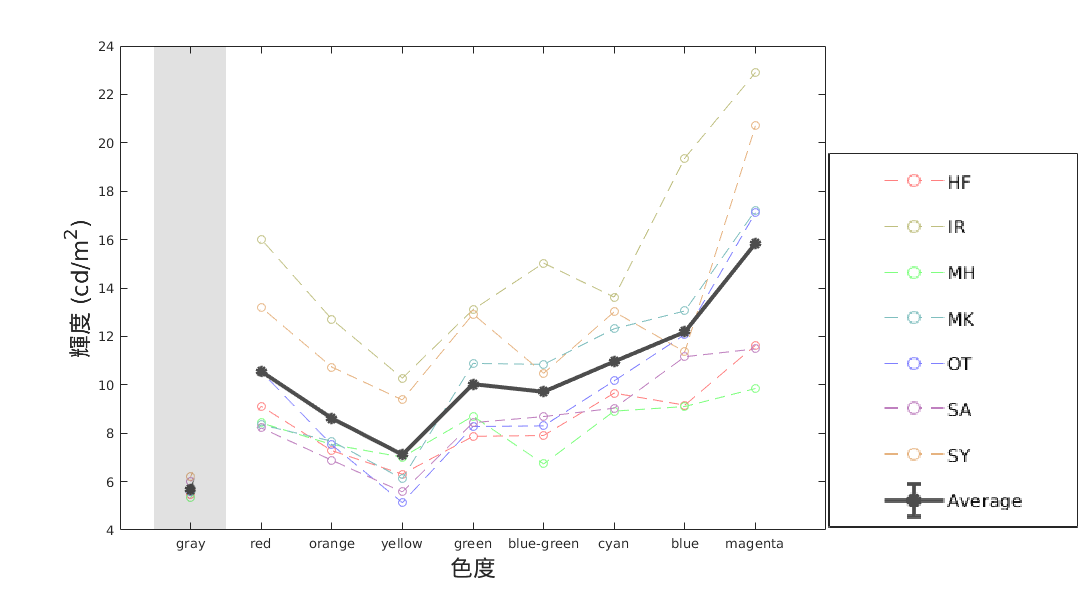
\includegraphics[width=14.0cm]{./img/ex2_res_SD_p.png}
                \caption{SD平均条件におけるテスト刺激の輝度}
                \label{ex2_SD}
            \end{figure}

            \begin{figure}[h]
                \centering
                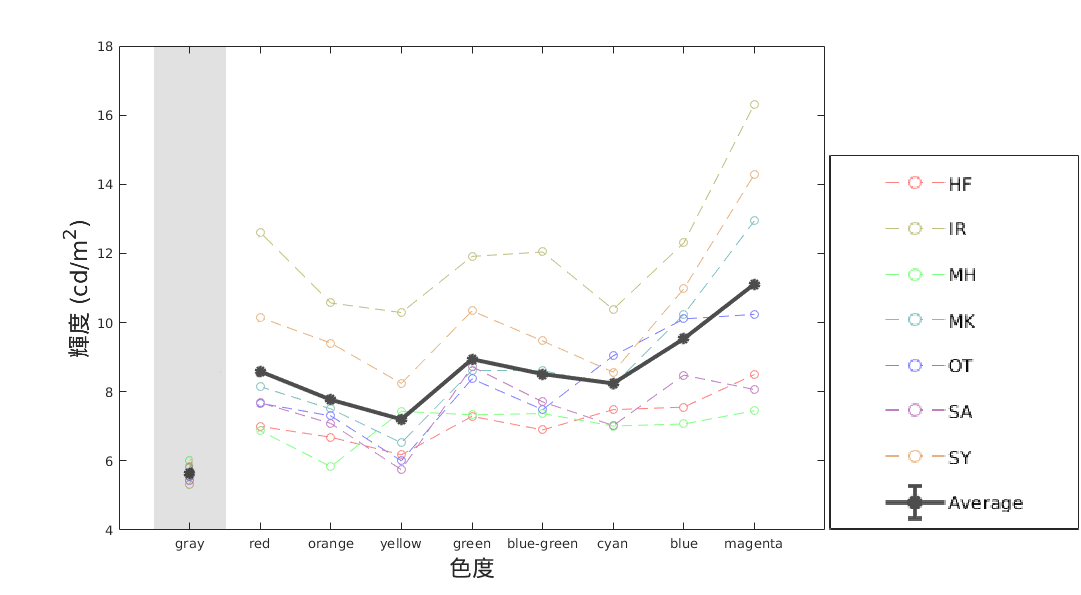
\includegraphics[width=14.0cm]{./img/ex2_res_D_p.png}
                \caption{D平均条件におけるテスト刺激の輝度}
                \label{ex2_D}
            \end{figure}


            図\ref{ex2_SD}と図\ref{ex2_D}に各被験者と被験者間平均のテスト刺激の輝度を示す.
            どちらの条件においても,magentaの明るさが非常に大きく,grayに次いでyellowの明るさが小さかった.
            被験者間では,SD条件,D条件共に色度に対する応答の傾向に大きな違いは見られなかった.
            また,有彩色のテスト刺激の輝度値は,全体的にD条件よりSD条件の方が大きかった.

            本実験により,実験1で用いた刺激の平均色のHK効果を定量化した.
            次に,この結果と実験1の結果から,光沢感と明るさの関連性を検証する.

    \newpage
        \subsection{実験1との関連性}

            \begin{figure}[h]
                \centering
                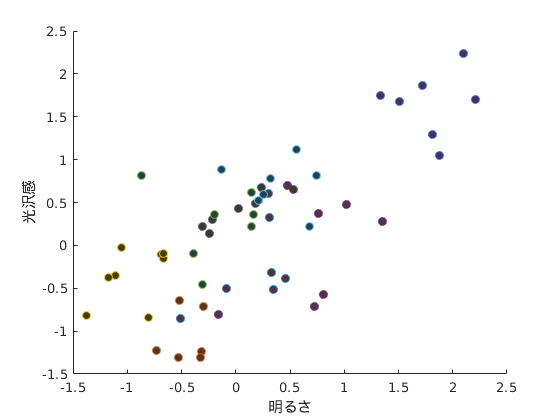
\includegraphics[width=12.0cm]{./img/ex3_DSD.png}
                \caption{Dragon形状のSD条件における散布図}
                \label{ex3_DSD}
            \end{figure}

            \begin{figure}[h]
                \centering
                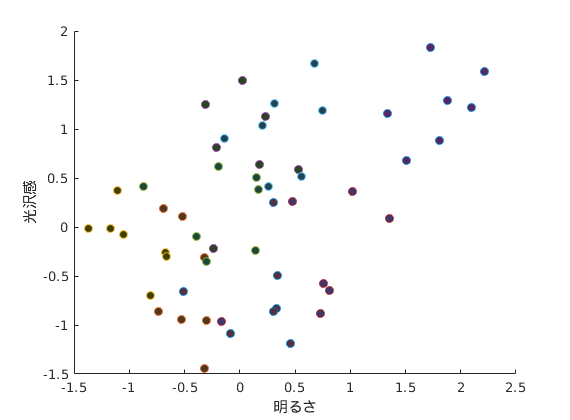
\includegraphics[width=12.0cm]{./img/ex3_BSD.png}
                \caption{Bunny形状のSD条件における散布図}
                \label{ex3_DSD}
            \end{figure}

            \begin{figure}[h]
                \centering
                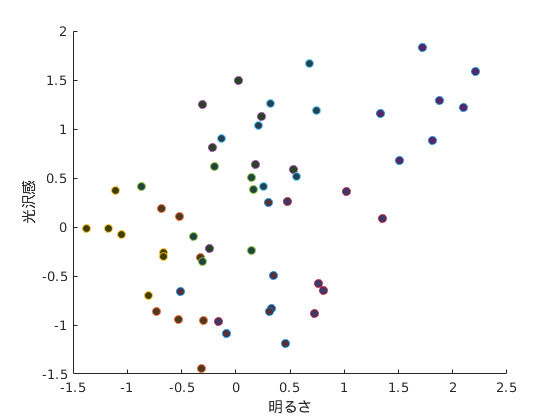
\includegraphics[width=12.0cm]{./img/ex3_DD.png}
                \caption{Dragon形状のD条件における散布図}
                \label{ex3_DD}
            \end{figure}

            \begin{figure}[h]
                \centering
                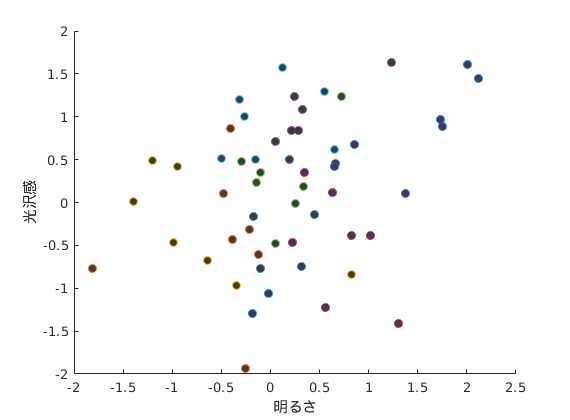
\includegraphics[width=12.0cm]{./img/ex3_BD.png}
                \caption{Bunny形状のD条件における散布図}
                \label{ex3_BD}
            \end{figure}

            \begin{table}[h]
                \centering
                \caption{各条件における実験1と実験2の結果の相関係数}
                \begin{tabular}{|l||c|c|} \hline
                                & SD       & D        \\ \hline \hline
                    Dragon      & 0.8828   & 0.8290   \\ \hline
                    Bunny       & 0.6490   & 0.5184   \\ \hline
                \end{tabular}
                \label{cc}
            \end{table}

            図\ref{ex3_DSD}から図\ref{ex3_BD}は,実験1と実験2のデータの両方に正規化を行い,物体形状と条件ごとに散布図にプロットしたものである.
            各点の色は実験で使われた9種類の色度からなり,横軸は明るさを,縦軸は光沢感を表す.
            また表\ref{cc}は各物体形状・着色条件における相関係数を表す.

            Dragon形状におけるSD条件,Dragon形状におけるD条件において比較的強い正の相関が見られたが,これに比べてBunny形状におけるSD条件,Bunny形状におけるD条件の相関係数は小さい値を示した.
            
        \subsection{考察}
        
            表\ref{cc}の結果は,H-K効果がもたらす知覚的な明るさは光沢感に寄与する要因の一つであるが,他の要因も寄与している可能性を示唆する.

    \newpage